\documentclass{article}

% Include useful packages
\usepackage{fullpage}
\usepackage{graphicx}
\usepackage{amsmath}
\usepackage{amssymb}
\usepackage{amsfonts}
\usepackage{color} 
\usepackage{fancyvrb}
\usepackage[sort, numbers]{natbib}
\usepackage{url}
\usepackage{subfigure}

\linespread{1.4}

% Helpful commands for authors' notes
\newcommand{\authornote}[2]{{\bf [#1: #2]}}
\newcommand{\alex}[1]{\authornote{Alex}{#1}}
\newcommand{\ozzy}[1]{\authornote{Ozzy}{#1}}
\newcommand{\highlight}[1]{{\color{red} \bf{#1}}}

\begin{document}

% Make title

\title{\highlight{Something like...} Comparing individual-based approaches to modelling the self-organization of multicellular tissues}

\author{James M. Osborne\footnotemark[3]\footnotemark[4]\footnotemark[2] \thanks{Corresponding author ({\tt James.Osborne@cs.ox.ac.uk})}\ 
\and Alexander G. Fletcher\footnotemark[5]\ \footnotemark[2] 
\and Daniel G. Harvey\footnotemark[3]
\and Joseph M. Pitt-Francis\footnotemark[3]
\and P.K. Maini\footnotemark[5] 
\and David J. Gavaghan\footnotemark[3]
\and \highlight{Also Jonathan? Anyone else?}}

\renewcommand{\thefootnote}{\fnsymbol{footnote}}
\footnotetext[2]{Joint first authors}
\footnotetext[3]{Computational Biology Group, Department of Computer Science, University of Oxford, Wolfson Building, Parks Road, Oxford, OX1 3QD, UK}
\footnotetext[4]{Computational Science Laboratory, Microsoft Research, 21 Station Road, Cambridge, CB1 2FB, UK}
\footnotetext[5]{Wolfson Centre for Mathematical Biology, Mathematical Institute, University of Oxford, Andrew Wiles Building, Radcliffe Observatory Quarter, Woodstock Road, Oxford, OX2 6GG, UK}
\renewcommand{\thefootnote}{\arabic{footnote}}

% Notice that the footnote marks begin with [2] because the first mark (the asterisk) will be used in the title for date-received information by SIAM, even if not already used for support data.

\maketitle

\begin{abstract}
\highlight{Which journal shall we submit to?}

\highlight{Please generate all results figures in both .png and .eps formats and in greyscale and colour versions for ease of editing etc.}
\end{abstract}

%%%%%%%%%%%%%%%%%%%%%%%%%%%%%%%%%%%%%%%%%%%%%%%%%%
%%%%%%%%%%%%%%%%%%%% Section %%%%%%%%%%%%%%%%%%%%%
%%%%%%%%%%%%%%%%%%%%%%%%%%%%%%%%%%%%%%%%%%%%%%%%%%

\section{Introduction} \label{sec:intro}

General motivation:
\begin{itemize}
\item Discuss the importance of understanding how cells behave and self-organise within biological tissues.
\item Describe how during morphogenesis and homeostasis, the repertoire of cell behaviours in response to biochemical and biophysical cues is limited to processes such as division, `respecification' (including differentiation and senescence), death, growth, migration, shape changes, and secretion or surface presentation of signalling molecules. Briefly discuss each of these processes in turn, providing concrete examples in each case.
\item Introduce the concept of individual-based models of cell populations and discuss merits over other `traditional' (i.e. continuum mean-field) models. Highlight past successes of this approach in advancing understanding of biological systems.
\item Spell out the huge variety of individual-based models and the lack of comparisons between approaches; the few examples of this include \citet{Galle2006Individual} and \citet{Osborne2010Hybrid}. How do the different individual-based models compare to one another?
\item Motivate the implementation of such models within a consistent computational framework when undertaking such a comparison, to avoid artifacts associated with different methods of numerical solution. Emphasize the lack of `benchmarks' for comparison.
\item Provide overview of structure of rest of paper.
\end{itemize}

%%%%%%%%%%%%%%%%%%%%%%%%%%%%%%%%%%%%%%%%%%%%%%%%%%
%%%%%%%%%%%%%%%%%%%% Section %%%%%%%%%%%%%%%%%%%%%
%%%%%%%%%%%%%%%%%%%%%%%%%%%%%%%%%%%%%%%%%%%%%%%%%%
\section{Review of different modelling approaches}\label{sec:discrete_models}
Review the various individual-based approaches to modelling cell populations:
\begin{itemize}
\item Lattice-based models: cellular automata and the cellular Potts model. Off-lattice models: centre-based models (`overlapping spheres' and Voronoi tessellation) and vertex-based models. Other models, such as the subcellular element model; it might be worth highlighting the `symmetry' of the four types of model we consider in this paper (centre-based as an off-lattice analogue of CA, vertex-based as an off-lattice analogue of CPM), since this indicates why we haven't also considered e.g. the SEM. Relevant references: \citet{Fletcher2013Implementing, Fletcher2014Vertex} for vertex-based models, perhaps \citet{VossBohme2012Mulit-scale} for the cellular Potts model.
\item Approaches to coupling such models to processes at different spatial scales: models that are coupled to continuum descriptions of transport processes; and models that are coupled to detailed representations of subcellular phenomena.
\item Include the underlying mathematics at a level sufficient to allow comparison, but wherever possible refer to relevant literature for full details.
\end{itemize} 

\noindent List existing codes: Chaste, CompuCell3d, Morpheus, EPISIM, CellSys, VirtualLeaf, Biocellion, Drasdo's code, MultiCellXML, ...

\noindent Discuss the technical implementation of such models:
\begin{itemize}
\item To what extent are the codes used to simulate such models open source, well documented, fully validated, or able to link against other software?
\item Reiterate that to accurately compare these models we need to implement them in a consistent simulation framework.
\item Lead in to brief discussion of Chaste, relying on the recent technical papers as key references for further implementation details. We won't put any code or structure details as these are in the technical papers.
\end{itemize}

%%%%%%%%%%%%%%%%%%%%%%%%%%%%%%%%%%%%%%%%%%%%%%%%%%
%%%%%%%%%%%%%%%%%%%% Section %%%%%%%%%%%%%%%%%%%%%
%%%%%%%%%%%%%%%%%%%%%%%%%%%%%%%%%%%%%%%%%%%%%%%%%%
\section{Model comparison}\label{sec:model_comparison}
We now present a series of exemplar simulations to compare how the processes discussed in Section~\ref{sec:intro} are represented in each modelling framework.
More importantly we discuss how the differences in representation influence the results of the simulation. 
We use cell-based Chaste; see \citet{Mirams2013Chaste} and \citet{Pitt-Francis2012Chaste} for further details.

%%%%%%%%%%%%%%%%%%% SubSection %%%%%%%%%%%%%%%%%%%
\subsection{Adhesion} \label{sec:adhesion}

Discuss biological background:
\begin{itemize}
\item Discuss how if embryonic cells of two or more histological types are placed into contact with each other, they can undergo spontaneous reproducible patterns of rearrangement; this process of cell sorting can generate checkerboard patterns, engulfment of one cell type by another, or other more complex patterns. Describe the differential adhesion hypothesis, which states that cells tend to prefer cell-cell contact with certain cell types rather than others due to type-specific differential intercellular adhesion, and the differential surface contraction hypothesis, which states that each cell exhibits surface contraction and cells of different types exert different degrees of surface contraction when in contact with other cell types or any surrounding medium.
\end{itemize}

\noindent Summarize existing models:
\begin{itemize}
\item There are lots of cellular Potts model references for cell sorting. We may also want to touch on the crypt paper by \citet{Wong2010Computational}, which considers differential adhesion between crypt cells caused by the differential activation of EphB receptors and ephrinB ligands along the crypt axis, and sets up the crypt as a common thread running through the paper.
\item Describe Roeland Merk's recent work in this area.
\end{itemize}

\noindent Describe an example model of differential adhesion in a monolayer in the absence of proliferation or respecification:
\begin{itemize}
\item Compare results for each of the individual-based models using statistics such as fractional boundary length (the number of mismatched bonds between cells of type A and cells of type B, divided by the total number of mismatched bonds, as a function of time), total boundary length (the total number of mismatched bonds between neighbouring lattice sites, or off-lattice equivalent), total time needed for aggregates to sort completely as a function of the proportion of cells of type A (conditional on this happening), and the average fraction of type A neighbours around type B cells, as a function of time.
\item The idea behind this example is that the centre- and vertex-based models will evolve to a local minimum in the total energy of the system as they are updated deterministically. In contrast, the cellular automaton and cellular Potts model undergo repeated annealing due to their stochastic updating, and will eventually end up at the global minimum, even if it may not be biologically realistic.
\item This example demonstrates how Chaste deals with cell sorting, a process occurring at the cellular level.
\item \highlight{Make sure that we have described the technical details for each model clearly, as well as our method of numerical solution. 
What model(s) of cell division have we used?
Also spell out how we relate timescales between models, in particular between the cellular Potts model and the others.}
\end{itemize}

\noindent Extra functionality required for this example:
\begin{itemize}
\item Cell sorting in centre-based simulations - a new force class.
\item Cell sorting in CA simulations - a new update rule.
\item Output fractional boundary length - presumably through simulation modifiers and/or cell population writers.
\end{itemize}

\noindent Results - go through figures and draw some conclusions. 
\highlight{Where did the simulation snapshot figures go? 
Make sure that we also run each simulation to `steady state' to compare equilibrium configurations - presumably over a sufficiently long time the cellular Potts model will give you complete sorting, in contrast with e.g. the vertex model?}

\begin{figure}
\centering
\setlength{\unitlength}{1cm}
\subfigure[]{
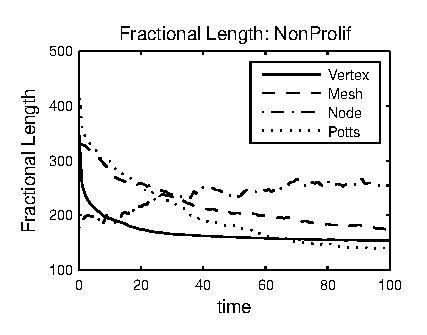
\includegraphics[width=6cm]{Figs/CellSorting/NonProlifFigs/FractionalLength}
\label{fig:CellSorting:a}
}
\subfigure[]{
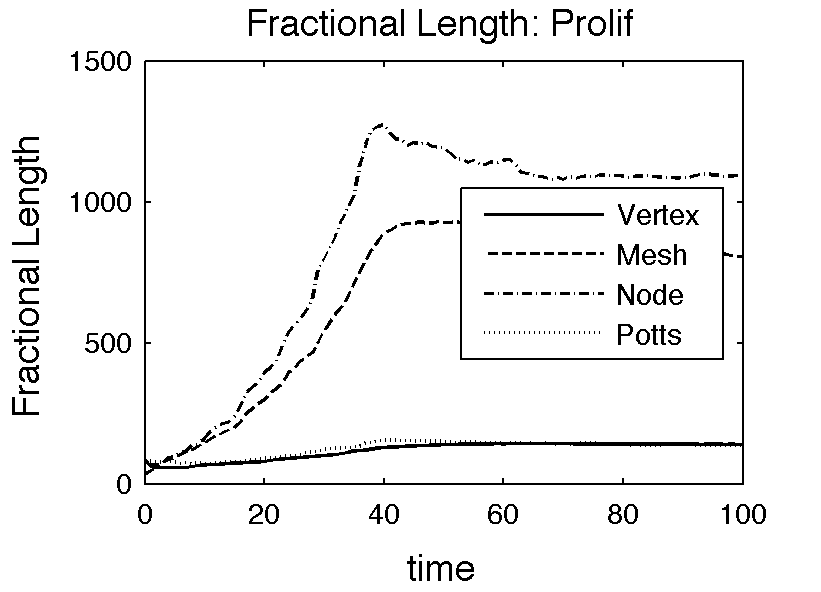
\includegraphics[width=6cm]{Figs/CellSorting/ProlifFigs/FractionalLength}
\label{fig:CellSorting:b}
}
\subfigure[]{
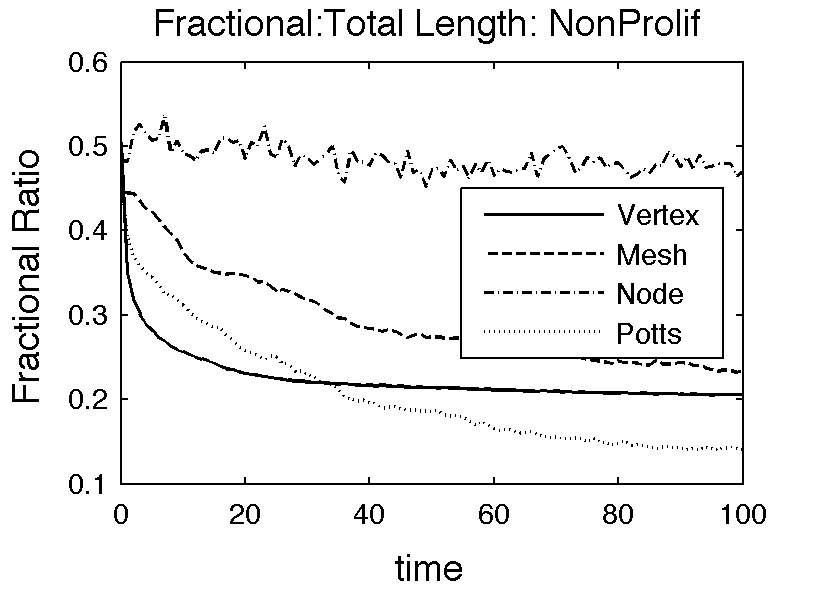
\includegraphics[width=6cm]{Figs/CellSorting/NonProlifFigs/FractionalLengthRatio}
\label{fig:CellSorting:c}
}
\subfigure[]{
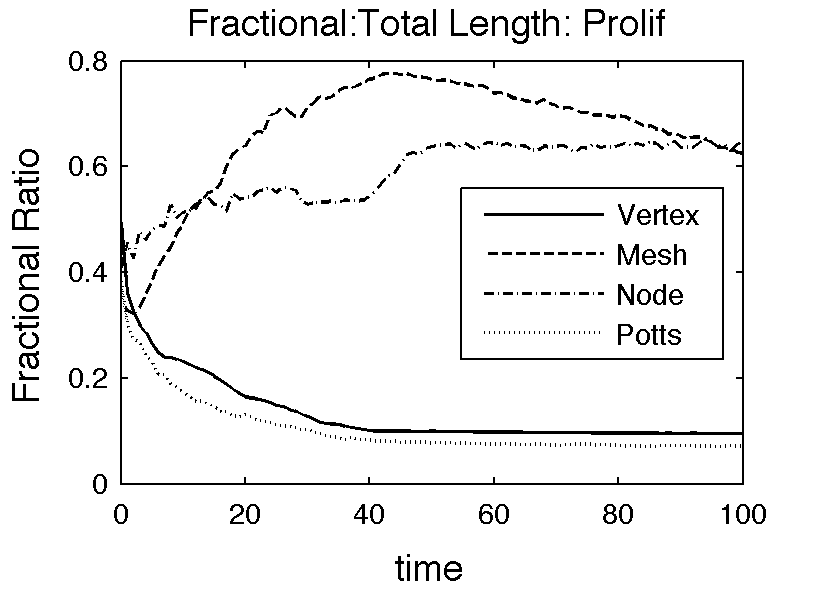
\includegraphics[width=6cm]{Figs/CellSorting/ProlifFigs/FractionalLengthRatio}
\label{fig:CellSorting:d}
}
\subfigure[]{
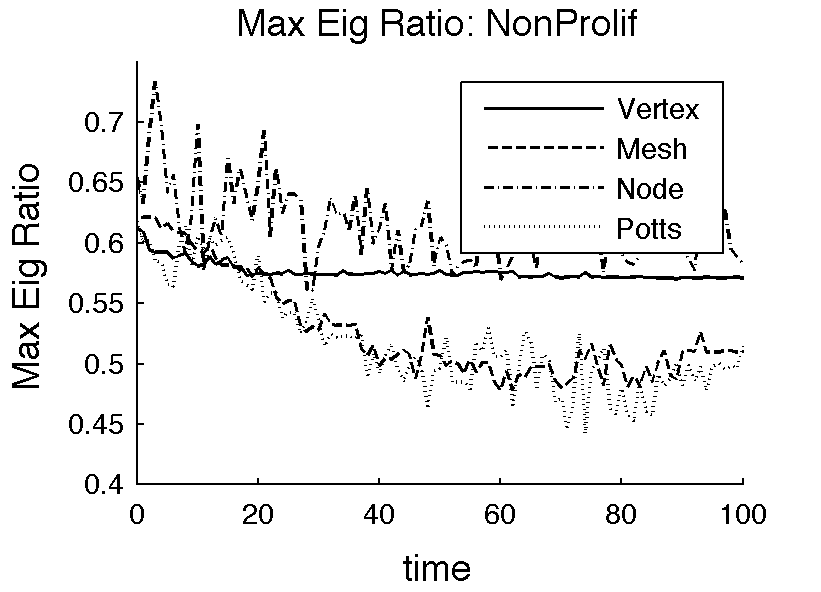
\includegraphics[width=6cm]{Figs/CellSorting/NonProlifFigs/MaxEigRatio}
\label{fig:CellSorting:e}
}
\subfigure[]{
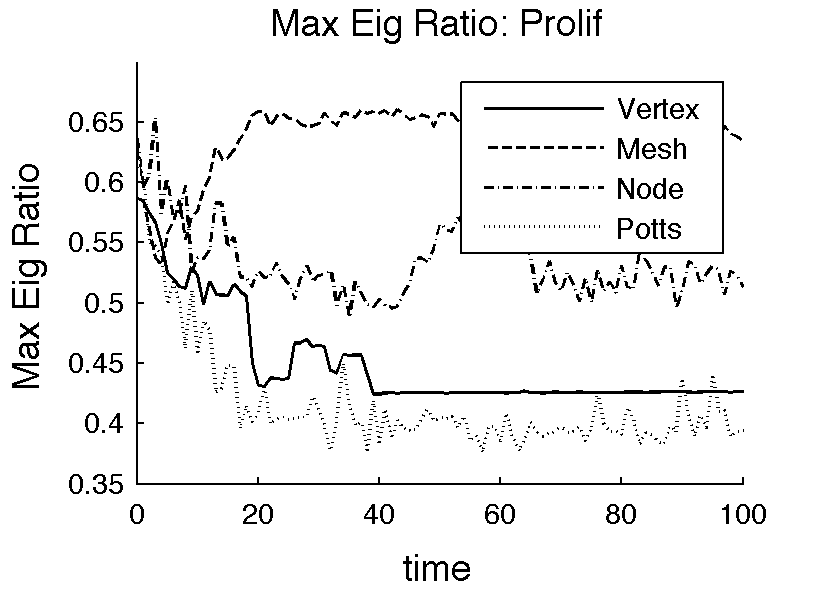
\includegraphics[width=6cm]{Figs/CellSorting/ProlifFigs/MaxEigRatio}
\label{fig:CellSorting:f}
}
\subfigure[]{
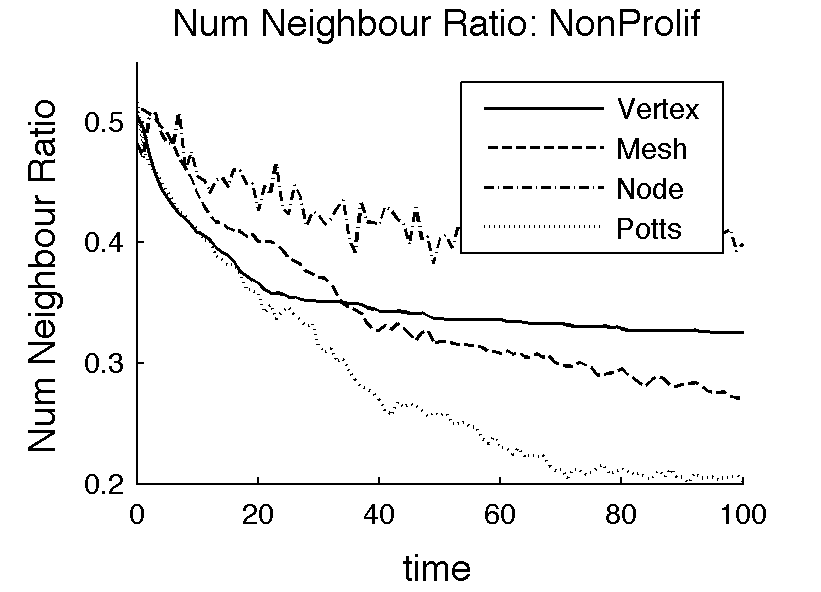
\includegraphics[width=6cm]{Figs/CellSorting/NonProlifFigs/NumNeighbourRatio}
\label{fig:CellSorting:g}
}
\subfigure[]{
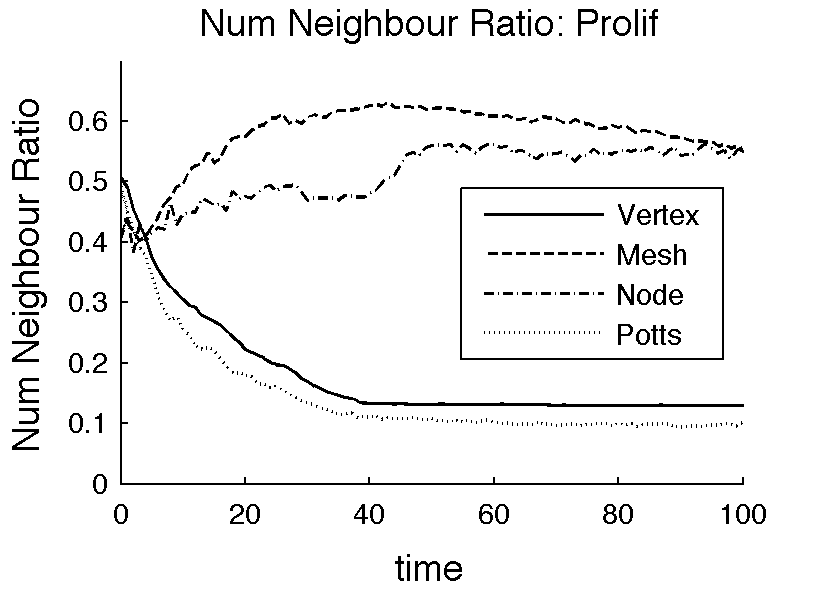
\includegraphics[width=6cm]{Figs/CellSorting/ProlifFigs/NumNeighbourRatio}
\label{fig:CellSorting:h}
}
\caption{(a)}
\label{fig:CellSorting}
\end{figure}

\highlight{Comments on Figure~\ref{fig:CellSorting}: 
Repace the title above each subfigure in the left column with just `Without cell divisions' and the title above each subfigure in the right column with just `With cell divisions' (or just remove the subfigure titles completely).
Remove legend from each subfigure as unnecessary duplication, instead just state which lines correspond to which models in the caption. 
Make all font sizes a bit larger. 
x-axis: ``time" should read ``Time". 
What are the units? If everything is non-dimensionalised, make sure to say this in the main text. 
Please define each of the quantities that you are plotting on each row. 
General comment: ``Mesh" and ``Node" are probably better named as something like ``Delaunay triangulation" and "Overlapping spheres" (or abbreviation) respectively, in order to be a bit less Chaste-specific and clearer for the audience.}

%%%%%%%%%%%%%%%%%%% SubSection %%%%%%%%%%%%%%%%%%%
\subsection{Proliferation, death and differentiation} \label{sec:proliferation}

Discuss biological background:
\begin{itemize}
\item Discuss patterns of cell proliferation, differentiation and apoptosis during development and homeostasis. Touch on intestinal homeostasis as a prime example of this.
\item Describe the phenomenon of contact inhibition (or density-dependent inhibition) of cell division, i.e. growth saturation at high cell densities, which is believed to protect the viability of cells in tissues by preventing over-proliferation. Briefly discuss how contact inhibition is governed by transmembrane proteins called cadherins, which act as mechanotransducers.
\item Explain how in the intestinal crypt some form of contact inhibition may operate, in which cells at the base of the crypt do not proliferate at their maximal rate due to overcrowding, giving rise to a complex pattern of cell proliferation up the crypt.
\end{itemize}

\noindent Summarize existing models:
\begin{itemize}
\item Lots of individual-based models consider the effect of spatial structure on patterns of cell proliferation and differentiation. In the context of the crypt, there are all the models stemming from \citet{Meineke2001Cell}.
\item Discrete models that consider the role of contact inhibition include \citet{Drasdo2003Individual}, \citet{Drasdo2007Role}, \citet{Galle2005Modeling}, and possibly Fletcher (2010) and Sara-Jane's crypt paper.
\end{itemize}

\noindent Describe an example model of contact inhibition of cell division in an established model of a colonic crypt:
\begin{itemize}
\item Describe the simple cylindrical crypt geometry used in \citet{vanLeeuwen2009Integrative, Osborne2010Hybrid, Mirams2012Theoretical}. Relate this to Sara-Jane's crypt model, which includes contact inhibition of cell proliferation.
\item Compare results for each of the individual-based models using velocity profiles, as done in the case of centre- and vertex-based models by \citet{Osborne2010Hybrid}.
\item The idea behind this example is that all individual-based models should be very similar when considering a `position-based' cell-cycle model (in which cell proliferation occurs below a threshold height up the crypt, corresponding to a threshold Wnt stimulus). However the individual-based models should exhibit different behaviour when incorporating contact inhibition of cell proliferation into the cell-cycle model.
\item This example demonstrates how Chaste includes coupling of cell-level processes to simple subcellular processes and deals with cell proliferation, death and differentiation.
\end{itemize}

\noindent Extra functionality required for this example:
\begin{itemize}
\item Set up a CA simulation of a crypt; possibly see also the model by \citet{Paulus1992Model}. 
\item Decide on how to implement contact inhibition in a CA model as the area is always 1; we could consider multiple occupancy CA or use the density of neighbours to specify contact inhibition.
\item Extend \texttt{ContactInhibitionCellCycleModel} to work with on-lattice simulations. This will require a \texttt{VolumeTrackedOnLatticeSimulation} analagous to the \texttt{VolumeTrackedOffLatticeSimulation} class. 
\highlight{Out of date - presumably we use simulation modifiers now?}
\end{itemize}

\noindent Results - go through figures and draw some conclusions.

\begin{figure}
\centering
\setlength{\unitlength}{1cm}
\subfigure[]{
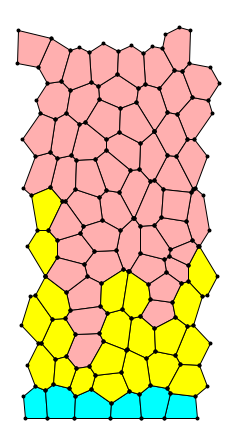
\includegraphics[width=3cm]{Figs/CylindricalCrypt/FigsNormal/Vertex100}
\label{fig:CylindricalCrypt:a}
}
\subfigure[]{
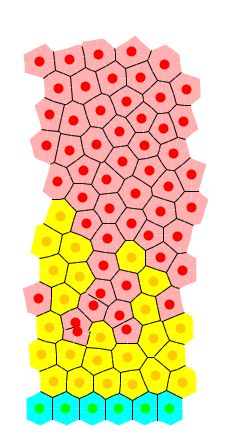
\includegraphics[width=3cm]{Figs/CylindricalCrypt/FigsNormal/Mesh100}
\label{fig:CylindricalCrypt:b}
}
\subfigure[]{
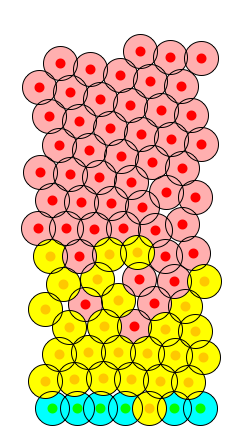
\includegraphics[width=3cm]{Figs/CylindricalCrypt/FigsNormal/Node100}
\label{fig:CylindricalCrypt:c}
}
\subfigure[]{
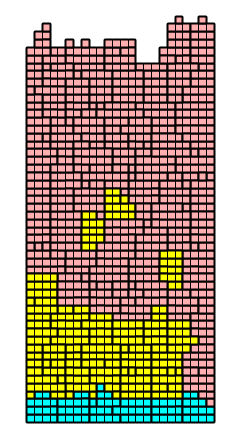
\includegraphics[width=3cm]{Figs/CylindricalCrypt/FigsNormal/Potts100}
\label{fig:CylindricalCrypt:d}
}
\subfigure[]{
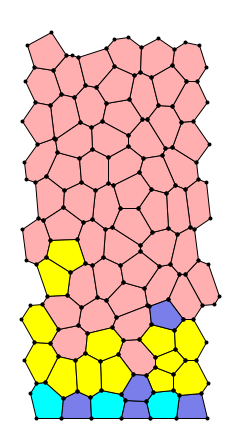
\includegraphics[width=3cm]{Figs/CylindricalCrypt/FigsCI/Vertex400}
\label{fig:CylindricalCrypt:e}
}
\subfigure[]{
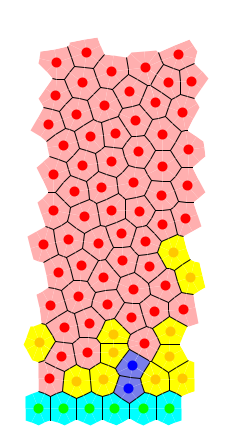
\includegraphics[width=3cm]{Figs/CylindricalCrypt/FigsCI/Mesh403}
\label{fig:CylindricalCrypt:f}
}
\subfigure[]{
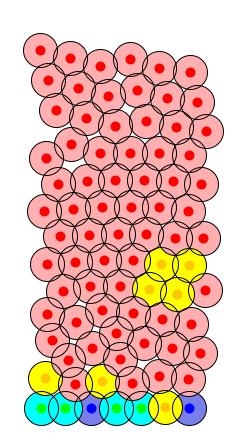
\includegraphics[width=3cm]{Figs/CylindricalCrypt/FigsCI/Node400}
\label{fig:CylindricalCrypt:g}
}
\subfigure[]{
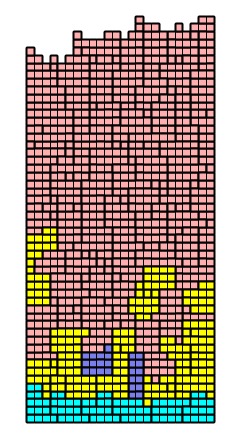
\includegraphics[width=3cm]{Figs/CylindricalCrypt/FigsCI/Potts401}
\label{fig:CylindricalCrypt:h}
}
\caption{(a)-(d) Generation Based Cell Cycle Model. (e)-(h) Contact Inhibition cell Generation based cell cycle model.}
\label{fig:CylindricalCrypt}
\end{figure}

\highlight{Comments on Figure~\ref{fig:CylindricalCrypt}: 
Where did the CA crypt model go? There are such models in the literature so I think it would be nice to include in this example. 
Same comment re: other case studies. 
The crypt geometries are unrealistically small - suggest we use established geometries as per \citet{Mirams2012Theoretical}. 
What does purple signify in these images? 
The cellular Potts model simulation snapshots are quite dark, I think because of the interior boundaries being drawn in black - it would be nice if only cell boundaries were drawn in black - is this possible?
}

\begin{figure}
\centering
\setlength{\unitlength}{1cm}
\subfigure[]{
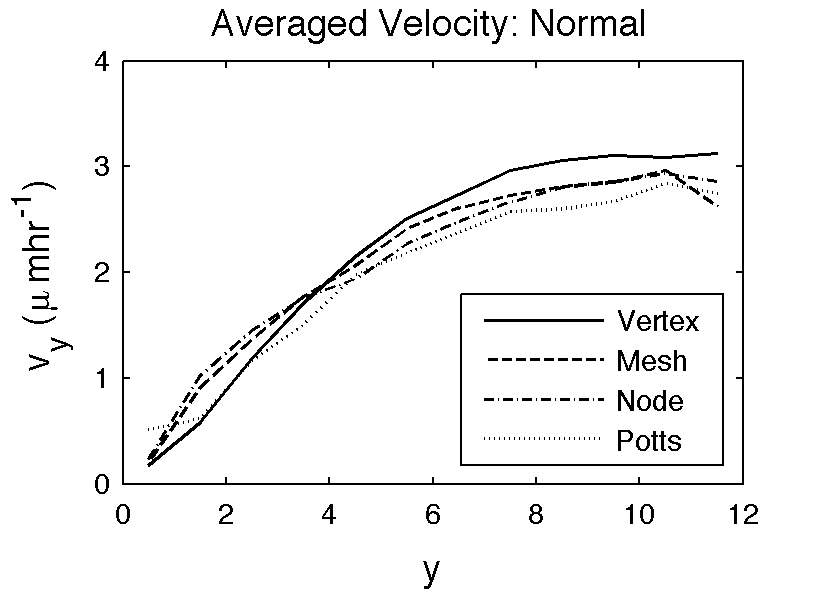
\includegraphics[width=6cm]{Figs/CylindricalCrypt/FigsNormal/HomeostasisCryptVelocityComparison}
\label{fig:CryptStats:a}
}
\subfigure[]{
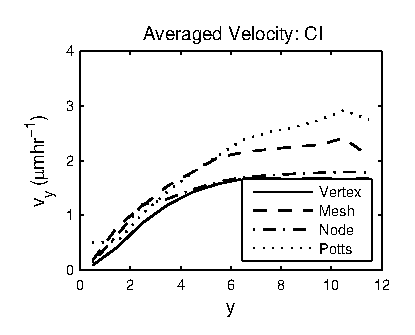
\includegraphics[width=6cm]{Figs/CylindricalCrypt/FigsCI/HomeostasisCryptVelocityComparison}
\label{fig:CryptStats:b}
}
\subfigure[]{
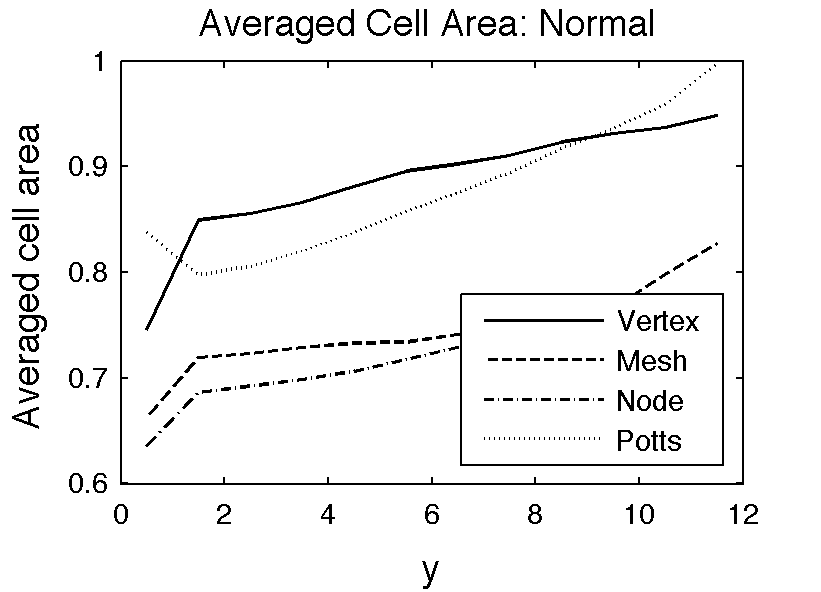
\includegraphics[width=6cm]{Figs/CylindricalCrypt/FigsNormal/HomeostasisCryptAveragedAreaComparison}
\label{fig:CryptStats:c}
}
\subfigure[]{
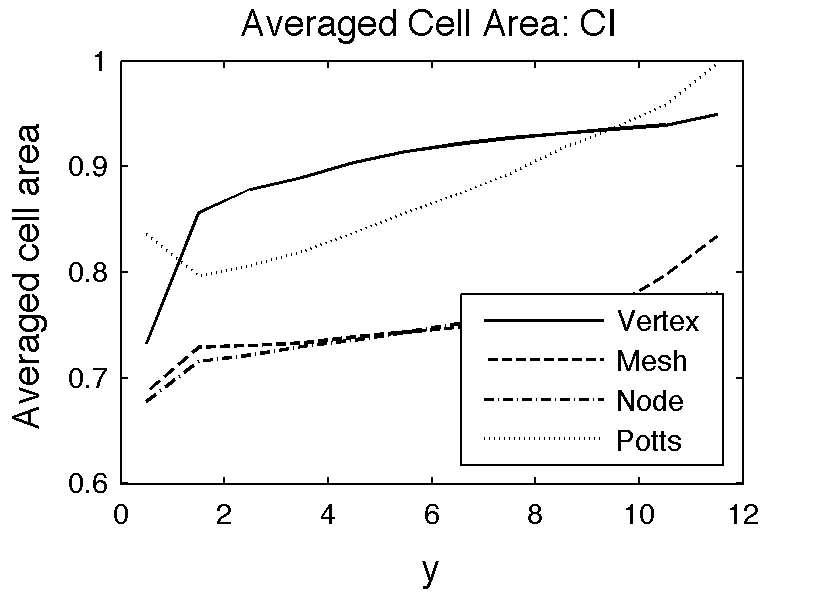
\includegraphics[width=6cm]{Figs/CylindricalCrypt/FigsCI/HomeostasisCryptAveragedAreaComparison}
\label{fig:CryptStats:d}
}
\subfigure[]{
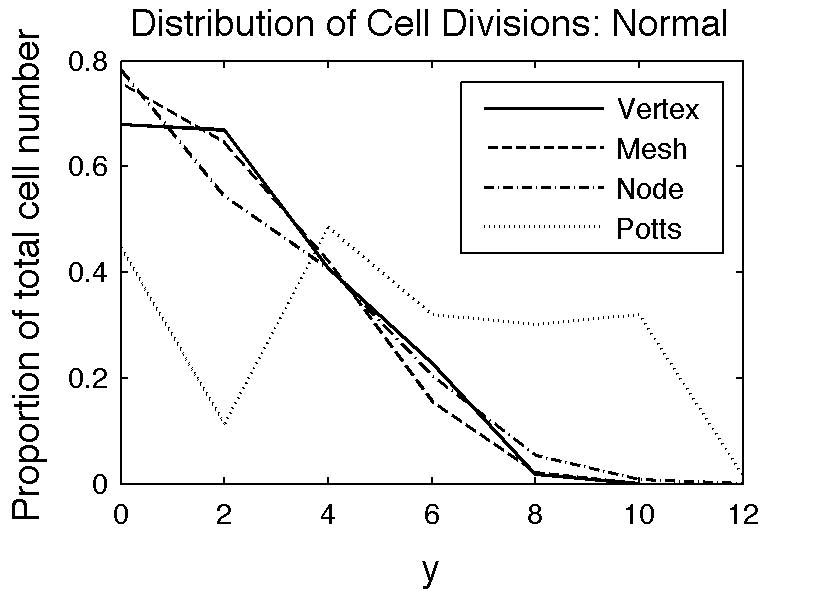
\includegraphics[width=6cm]{Figs/CylindricalCrypt/FigsNormal/CellDivisionDistributionComparison}
\label{fig:CryptStats:e}
}
\subfigure[]{
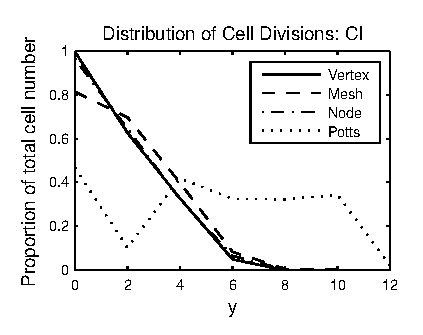
\includegraphics[width=6cm]{Figs/CylindricalCrypt/FigsCI/CellDivisionDistributionComparison}
\label{fig:CryptStats:f}
}
\subfigure[]{
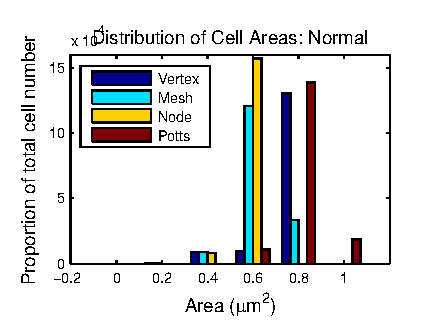
\includegraphics[width=6cm]{Figs/CylindricalCrypt/FigsNormal/CellAreaDistributionComparison}
\label{fig:CryptStats:g}
}
\subfigure[]{
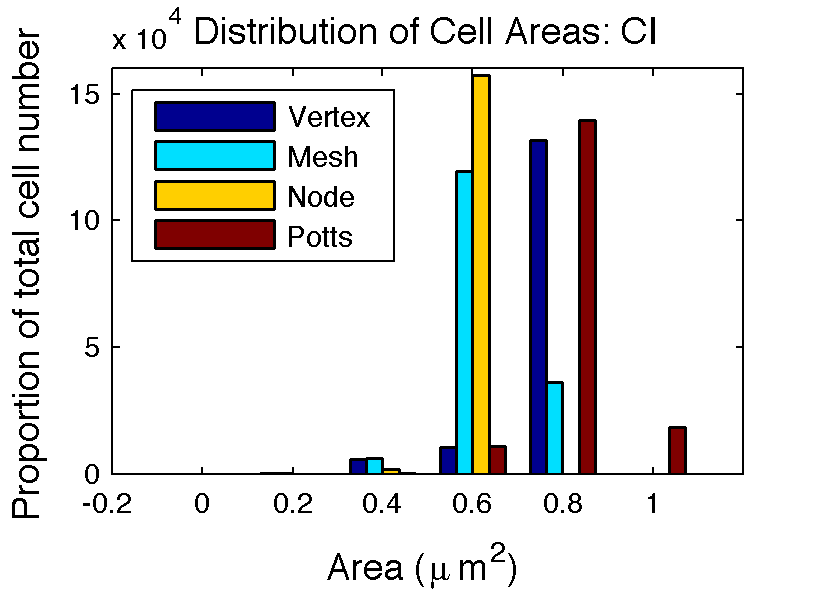
\includegraphics[width=6cm]{Figs/CylindricalCrypt/FigsCI/CellAreaDistributionComparison}
\label{fig:CryptStats:h}
}
\caption{(a)}
\label{fig:CryptStats:metrics}
\end{figure}

\highlight{Comments on Figure~\ref{fig:CryptStats:metrics}: 
Repace the title above each subfigure in the left column with just `Without contact inhbition' and the title above each subfigure in the right column with just `With contact inhibition' (or just remove the subfigure titles completely). 
Rename the x-axis in each subfigure to `Height up crypt' or whatever it is. Similar comments re: y-axis on top row. 
No need for subfigure legends - see similar comment about earlier figure. 
Please can we have greyscale versions of (g) and (h). 
Why are the proportions given as multiples of $10^4$ in (g) and (h)? 
Is each subfigure generated for a crypt in dynamic equilbrium? 
If so, we need to say this and say how this is defined (or do we just simulate each model up to some arbitrary time)? 
For (a) to (f), presumably the data are being binned? Need to say how this is done. 
Also maybe use finer bins - these graphs look quite `jagged'.
}

%%%%%%%%%%%%%%%%%%% SubSection %%%%%%%%%%%%%%%%%%%
\subsection{Short-range signalling} \label{sec:juxtacrine}

Discuss biological background:
\begin{itemize}
\item Brief description of lateral inhibition as a juxtacrine pattern-forming mechanism employed during morphogenesis. Focus on the action of the transmembrane proteins Notch and Delta, and their homologues, in mediating lateral inhibition and determining cell fate.
\item List particular biological systems featuring this process, e.g. {\it Drosophila} eye development, somitogenesis in vertebrates, and cell lineage specification in the mammalian gut.
\end{itemize}

\noindent Summarize existing models:
\begin{itemize}
\item Focus on discrete models of lateral inhibition: \citet{Collier1996Pattern, Owen1998Mathematical, Wearing2001Nonlinear, Webb2004Oscillations}. These models study conditions for fine-grained patterns in a fixed cell population; proliferation and differentiation are not considered. Possible aside on continuum and coarse-grained models, e.g. \citet{ODea2011Continuum}
\item More detailed models focusing on the intestine: \citet{Buske2011Comprehensive, Pin2012Modelling}. These models couple cell fate determination to Notch activity. Opportunity for linking back to previous crypt example (and mentioning Sophie's work if published and relevant).
\item Need to check if any cellular Potts models have considered Delta/Notch signalling.
\end{itemize}

\noindent Describe an example model of Delta/Notch signalling in a growing monolayer, with cell proliferation dependent on Delta levels:
\begin{itemize}
\item Compare results for each of the individual-based models using spatial descriptive statistics.
\item The idea is that the tissue level statistics will be different due to connectivity in models; this should result in different growth rates for the tissues.
\item The example demonstrates the inclusion of ODE-based subcellular models and also how to sense the local environment within the cell-based Chaste framework.
\end{itemize}

\noindent All the functionality needed for this example already exists in Chaste.

\begin{figure}
\centering
\setlength{\unitlength}{1cm}
\subfigure[]{
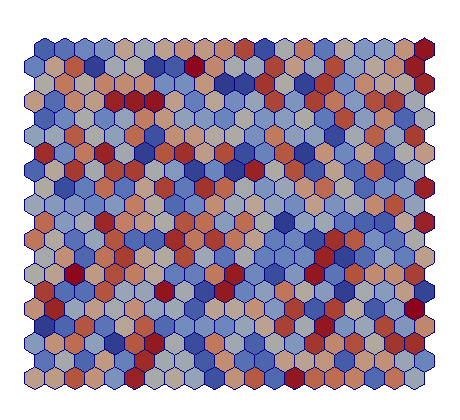
\includegraphics[width=3.7cm]{Figs/DeltaNotch/NonProlif/Vertex0}
\label{fig:DeltaNotchNonProlif:a}
}
\subfigure[]{
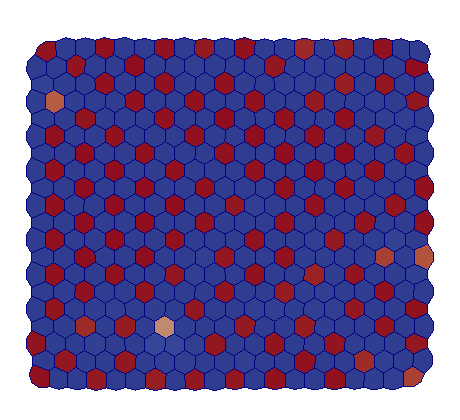
\includegraphics[width=3.7cm]{Figs/DeltaNotch/NonProlif/Vertex25}
\label{fig:DeltaNotchNonProlif:b}
}
\subfigure[]{
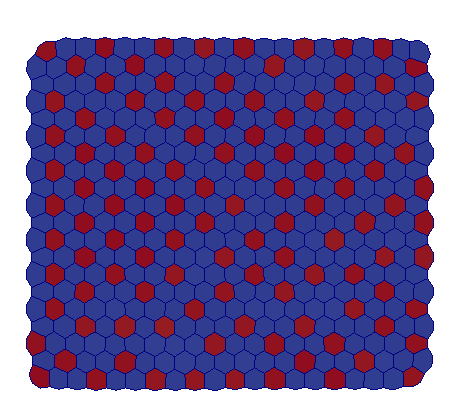
\includegraphics[width=3.7cm]{Figs/DeltaNotch/NonProlif/Vertex50}
\label{fig:DeltaNotchNonProlif:c}
}
\subfigure[]{
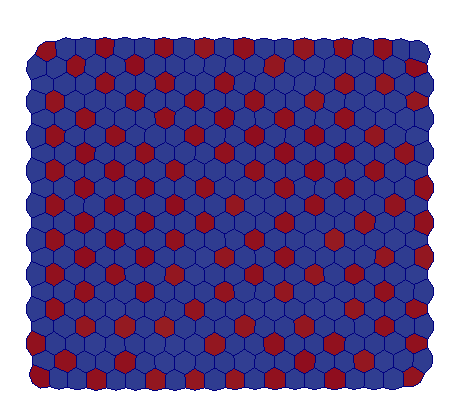
\includegraphics[width=3.7cm]{Figs/DeltaNotch/NonProlif/Vertex100}
\label{fig:DeltaNotchNonProlif:d}
}
\subfigure[]{
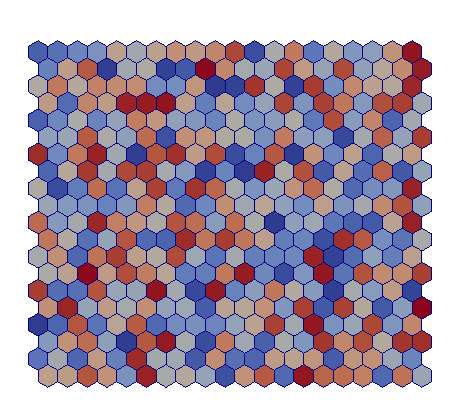
\includegraphics[width=3.7cm]{Figs/DeltaNotch/NonProlif/Mesh0}
\label{fig:DeltaNotchNonProlif:e}
}
\subfigure[]{
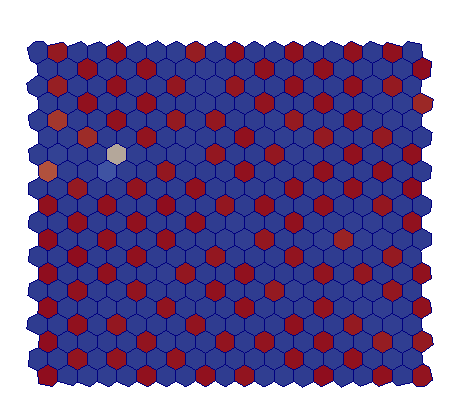
\includegraphics[width=3.7cm]{Figs/DeltaNotch/NonProlif/Mesh25}
\label{fig:DeltaNotchNonProlif:f}
}
\subfigure[]{
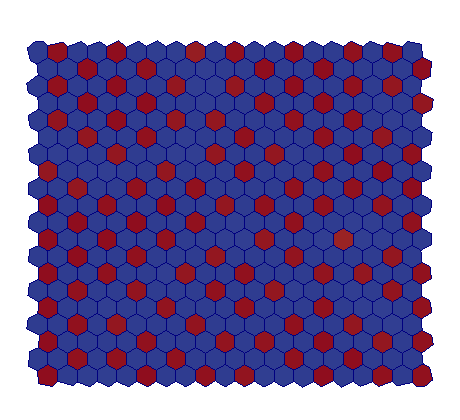
\includegraphics[width=3.7cm]{Figs/DeltaNotch/NonProlif/Mesh50}
\label{fig:DeltaNotchNonProlif:g}
}
\subfigure[]{
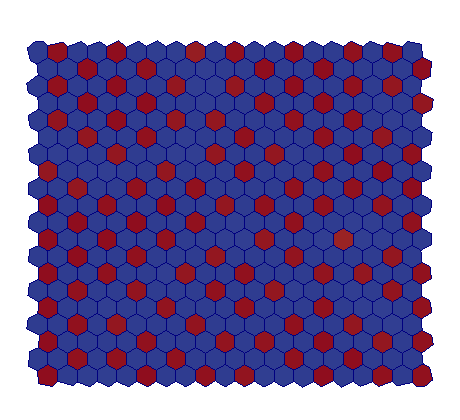
\includegraphics[width=3.7cm]{Figs/DeltaNotch/NonProlif/Mesh100}
\label{fig:DeltaNotchNonProlif:h}
}
\subfigure[]{
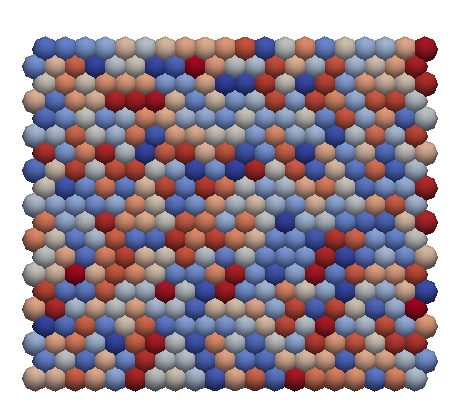
\includegraphics[width=3.7cm]{Figs/DeltaNotch/NonProlif/Node0}
\label{fig:DeltaNotchNonProlif:i}
}
\subfigure[]{
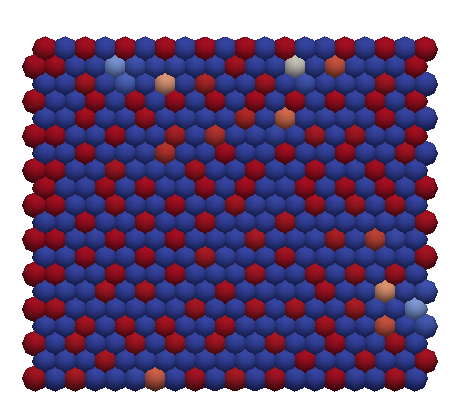
\includegraphics[width=3.7cm]{Figs/DeltaNotch/NonProlif/Node25}
\label{fig:DeltaNotchNonProlif:j}
}
\subfigure[]{
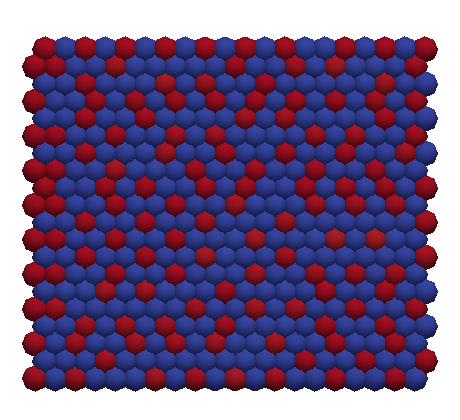
\includegraphics[width=3.7cm]{Figs/DeltaNotch/NonProlif/Node50}
\label{fig:DeltaNotchNonProlif:k}
}
\subfigure[]{
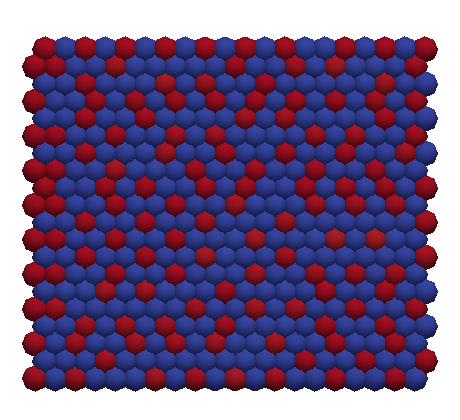
\includegraphics[width=3.7cm]{Figs/DeltaNotch/NonProlif/Node100}
\label{fig:DeltaNotchNonProlif:l}
}
\subfigure[]{
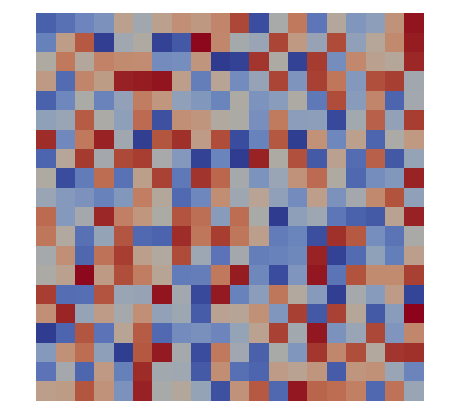
\includegraphics[width=3.7cm]{Figs/DeltaNotch/NonProlif/Potts0}
\label{fig:DeltaNotchNonProlif:m}
}
\subfigure[]{
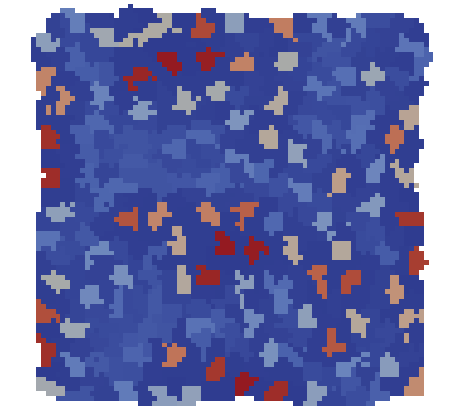
\includegraphics[width=3.7cm]{Figs/DeltaNotch/NonProlif/Potts25}
\label{fig:DeltaNotchNonProlif:n}
}
\subfigure[]{
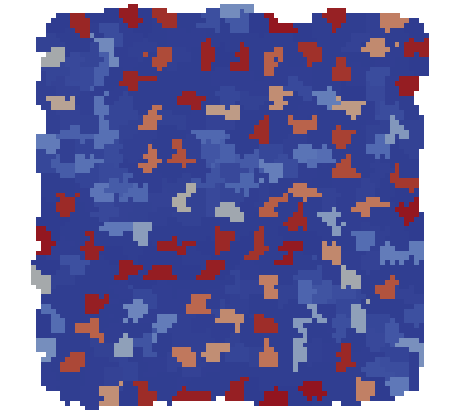
\includegraphics[width=3.7cm]{Figs/DeltaNotch/NonProlif/Potts50}
\label{fig:DeltaNotchNonProlif:o}
}
\subfigure[]{
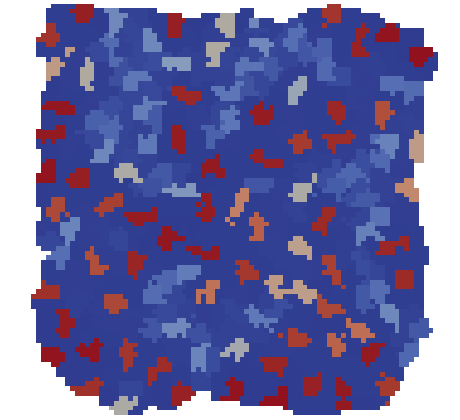
\includegraphics[width=3.7cm]{Figs/DeltaNotch/NonProlif/Potts100}
\label{fig:DeltaNotchNonProlif:p}
}
\caption{No Proliferation (a)-(d) VertexBased; (e)-(h) MeshBased; (i)-(l) Node Based; (m)-(p) Potts Based.}
\label{fig:DeltaNotchNonProlif}
\end{figure}

\highlight{Comments on Figure~\ref{fig:DeltaNotchNonProlif}: 
Subfigures (a) to (l) don't look very interesting - it seems like everything is pretty much at steady state by the second timepoint. 
Suggest plotting snapshots at earlier times so that there is some difference between (c) and (d), (g) and (h) and (k) and (l) respectively. 
We also need a colourbar and to clarify what is being visualised in each snapshot (delta or notch). 
Also, please can we have greyscale versions of each subfigure in case the target journal charges for colour images.
}

\begin{figure}
\centering
\setlength{\unitlength}{1cm}
\subfigure[]{
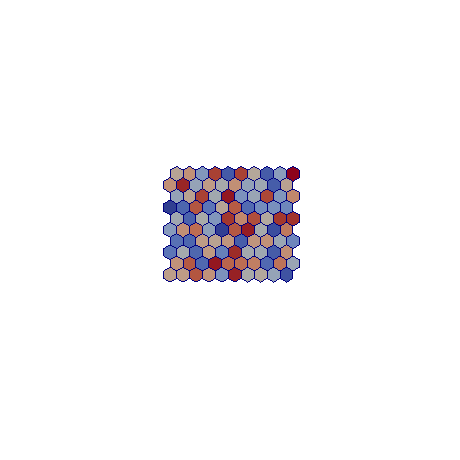
\includegraphics[width=3.7cm]{Figs/DeltaNotch/Prolif/Vertex0}
\label{fig:DeltaNotchProlif:a}
}
\subfigure[]{
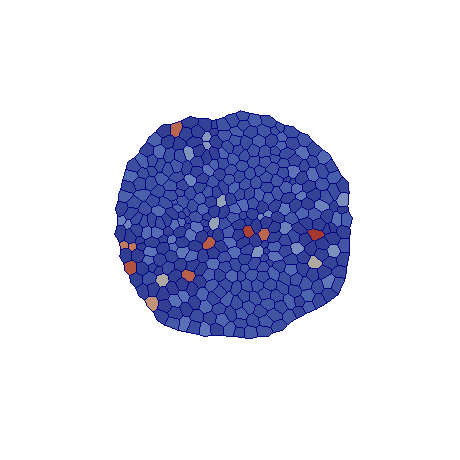
\includegraphics[width=3.7cm]{Figs/DeltaNotch/Prolif/Vertex25}
\label{fig:DeltaNotchProlif:b}
}
\subfigure[]{
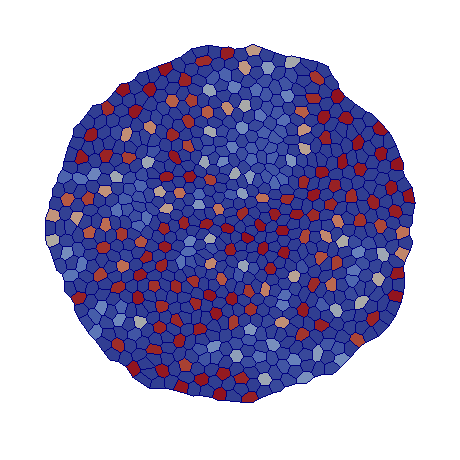
\includegraphics[width=3.7cm]{Figs/DeltaNotch/Prolif/Vertex50}
\label{fig:DeltaNotchProlif:c}
}
\subfigure[]{
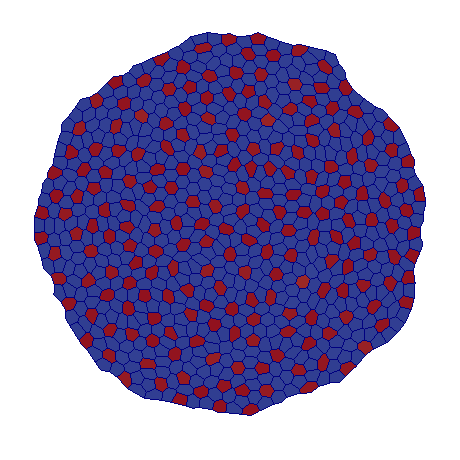
\includegraphics[width=3.7cm]{Figs/DeltaNotch/Prolif/Vertex100}
\label{fig:DeltaNotchProlif:d}
}
\subfigure[]{
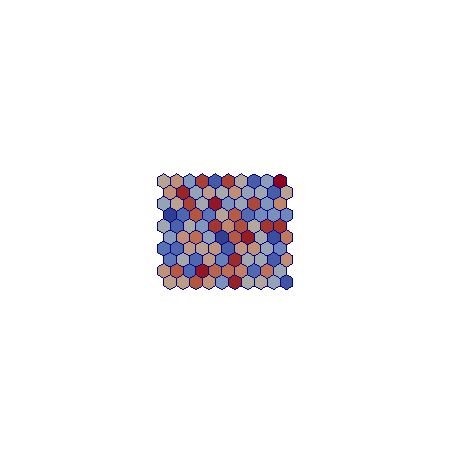
\includegraphics[width=3.7cm]{Figs/DeltaNotch/Prolif/Mesh0}
\label{fig:DeltaNotchProlif:e}
}
\subfigure[]{
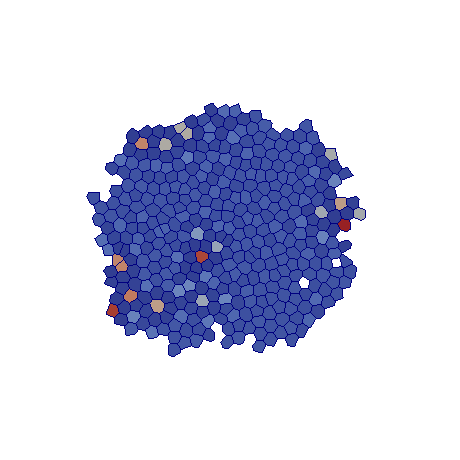
\includegraphics[width=3.7cm]{Figs/DeltaNotch/Prolif/Mesh25}
\label{fig:DeltaNotchProlif:f}
}
\subfigure[]{
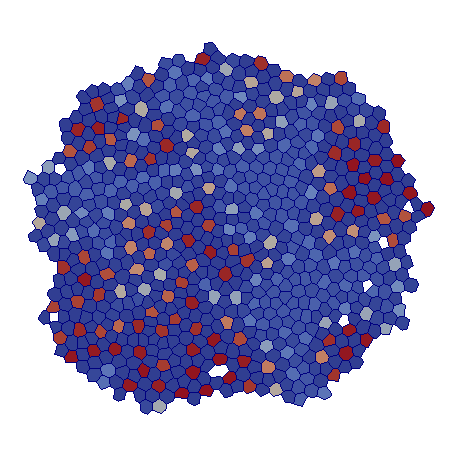
\includegraphics[width=3.7cm]{Figs/DeltaNotch/Prolif/Mesh50}
\label{fig:DeltaNotchProlif:g}
}
\subfigure[]{
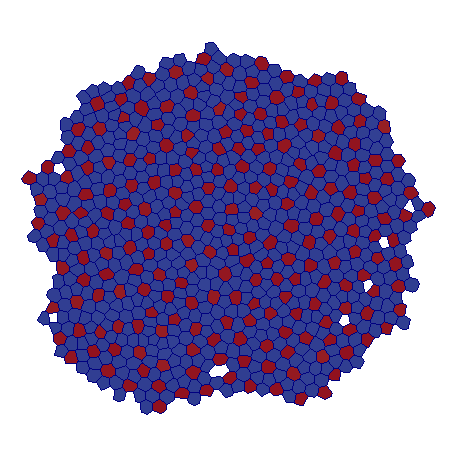
\includegraphics[width=3.7cm]{Figs/DeltaNotch/Prolif/Mesh100}
\label{fig:DeltaNotchProlif:h}
}
\subfigure[]{
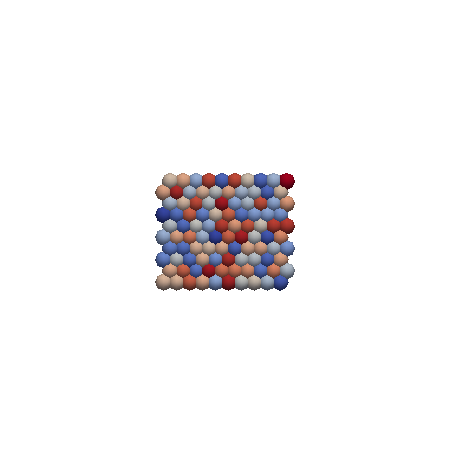
\includegraphics[width=3.7cm]{Figs/DeltaNotch/Prolif/Node0}
\label{fig:DeltaNotchProlif:i}
}
\subfigure[]{
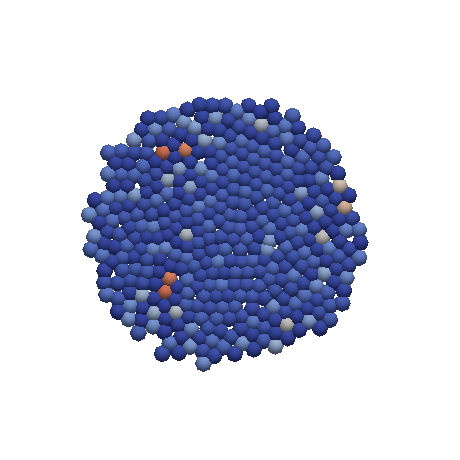
\includegraphics[width=3.7cm]{Figs/DeltaNotch/Prolif/Node25}
\label{fig:DeltaNotchProlif:j}
}
\subfigure[]{
\includegraphics[width=3.7cm]{Figs/DeltaNotch/Prolif/Node50}
\label{fig:DeltaNotchProlif:k}
}
\subfigure[]{
\includegraphics[width=3.7cm]{Figs/DeltaNotch/Prolif/Node100}
\label{fig:DeltaNotchProlif:l}
}
\subfigure[]{
\includegraphics[width=3.7cm]{Figs/DeltaNotch/Prolif/Potts0}
\label{fig:DeltaNotchProlif:m}
}
\subfigure[]{
\includegraphics[width=3.7cm]{Figs/DeltaNotch/Prolif/Potts25}
\label{fig:DeltaNotchProlif:n}
}
\subfigure[]{
\includegraphics[width=3.7cm]{Figs/DeltaNotch/Prolif/Potts50}
\label{fig:DeltaNotchProlif:o}
}
\subfigure[]{
\includegraphics[width=3.7cm]{Figs/DeltaNotch/Prolif/Potts100}
\label{fig:DeltaNotchProlif:p}
}
\caption{No Proliferation (a)-(d) VertexBased; (e)-(h) MeshBased; (i)-(l) Node Based; (m)-(p) Potts Based.}
\label{fig:DeltaNotchProlif}
\end{figure}

\highlight{Comments on Figure~\ref{fig:DeltaNotchProlif}: same comments apply as for Figure~\ref{fig:DeltaNotchNonProlif}. 
Also, subfigures (n) to (p) look weird - has something gone wrong here?
}

\begin{figure}
\centering
\setlength{\unitlength}{1cm}
\subfigure[]{
\includegraphics[width=6cm]{Figs/DeltaNotch/NonProlifPatternRatio}
\label{fig:DeltaNotchStats:a}
}
\subfigure[]{
\includegraphics[width=6cm]{Figs/DeltaNotch/ProlifPatternRatio}
\label{fig:DeltaNotchStats:b}
}
\caption{Ratio of Delta high cells to all cells for (a) no proliferation and  (b) with proliferation.}
\label{fig:DeltaNotchStats:metrics}
\end{figure}

\highlight{Comments on Figure~\ref{fig:DeltaNotchStats:metrics}: 
See earlier comments on subfigure titles and legends. 
Suggest we also compute spatial statistics such as Moran's I, Ripley's K etc. 
cf. Sophie's work.
}

%%%%%%%%%%%%%%%%%%% SubSection %%%%%%%%%%%%%%%%%%%
\subsection{Long-range signalling} \label{sec:morphagens}

Discuss biological background:
\begin{itemize}
\item Describe how morphgens are secreted signalling molecules that provide positional information to cells in a developing tissue and act as a trigger for cell growth, proliferation or differentiation. There are lots of examples and reviews relevant to this; see e.g. the recent review by \citet{Wartlick2011Understanding} discussing the insight that has been gained from studying the imaginal wing disc in {\it Drosophila}.
\end{itemize}

\noindent Summarize existing models:
\begin{itemize}
\item Again, lots of previous models; in terms of multiscale models, we should include references such as \citet{Schilling2011Cell}.
\end{itemize}

\noindent Describe an example model of a morphogen gradient influencing the development of an epithelial tissue: respecification:
\begin{itemize}
\item The idea behind this example is to set up a realistic geometry of e.g. an imaginal wing disc and to couple a reaction-diffusion PDE to cells secreting and taking up morphogen. Cells will proliferate based on morphogen level.
\item Compare results for each of the individual-based models using the resulting shapes of the tissue.
\item This example demonstrates morphogens being represented as reaction-diffusion systems coupled to the discrete cell level models in Chaste.
\end{itemize}

\noindent Extra functionality required for this example:
\begin{itemize}
\item Solving a single PDE on a vertex mesh - use cell centre to allow specification of a triangular mesh at each time step (see also \citet{Smith2011Incorporating}).
\item Solving a single PDE in an on-lattice simulation:
\begin{itemize}
\item either use lattice sites to specify a FE mesh and use this to solve the PDE;
\item or else implement a finite difference method for on-lattice simulations (this won't need the same level of detail as the FE solvers, just an \texttt{UpdateAfterSolve()} method in a new simulation class.
\end{itemize}
\end{itemize}

\highlight{Suggest we implement the simulation described in Section 7 of \citet{Smith2011Incorporating}.}
\begin{figure}
\centering
\setlength{\unitlength}{1cm}
\subfigure[]{
\includegraphics[width=3.7cm]{Figs/Monolayers/Vertex0}
\label{fig:MonolayersNonProlif:a}
}
\subfigure[]{
\includegraphics[width=5.0cm]{Figs/Monolayers/Vertex25}
\label{fig:MonolayersNonProlif:b}
}
\subfigure[]{
\includegraphics[width=5.0cm]{Figs/Monolayers/Vertex50}
\label{fig:MonolayersNonProlif:c}
}
\subfigure[]{
\includegraphics[width=5.0cm]{Figs/Monolayers/Mesh0}
\label{fig:MonolayersNonProlif:d}
}
\subfigure[]{
\includegraphics[width=5.0cm]{Figs/Monolayers/Mesh25}
\label{fig:MonolayersNonProlif:e}
}
\subfigure[]{
\includegraphics[width=5.0cm]{Figs/Monolayers/Mesh50}
\label{fig:MonolayersNonProlif:f}
}
\subfigure[]{
\includegraphics[width=5.0cm]{Figs/Monolayers/Node0}
\label{fig:MonolayersNonProlif:g}
}
\subfigure[]{
\includegraphics[width=5.0cm]{Figs/Monolayers/Node25}
\label{fig:MonolayersNonProlif:h}
}
\subfigure[]{
\includegraphics[width=5.0cm]{Figs/Monolayers/Node50}
\label{fig:MonolayersNonProlif:i}
}
\subfigure[]{
\includegraphics[width=5.0cm]{Figs/Monolayers/Potts0}
\label{fig:MonolayersNonProlif:j}
}
\subfigure[]{
\includegraphics[width=5.0cm]{Figs/Monolayers/Potts25}
\label{fig:MonolayersNonProlif:k}
}
\subfigure[]{
\includegraphics[width=5.0cm]{Figs/Monolayers/Potts50}
\label{fig:MonolayersNonProlif:l}
}
\caption{(a)-(c) VertexBased; (d)-(f) MeshBased; (g)-(i) Node Based; (j)-(l) Potts Based.}
\label{fig:Monolayers}
\end{figure}

\begin{figure}
\centering
\setlength{\unitlength}{1cm}
\subfigure[]{
\includegraphics[width=6cm]{Figs/Monolayers/NumCells}
\label{fig:DeltaNotchStats:a}
}
\subfigure[]{
\includegraphics[width=6cm]{Figs/Monolayers/NumLabeledCells}
\label{fig:DeltaNotchStats:b}
}
\caption{Number of cells (a) total number (b) number of labeled cells i.e. ones that absorb morphogen.}
\label{fig:DeltaNotchStats:metrics}
\end{figure}


%%%%%%%%%%%%%%%%%%%%%%%%%%%%%%%%%%%%%%%%%%%%%%%%%%
%%%%%%%%%%%%%%%%%%%% Section %%%%%%%%%%%%%%%%%%%%%
%%%%%%%%%%%%%%%%%%%%%%%%%%%%%%%%%%%%%%%%%%%%%%%%%%
\section{Discussion} \label{sec:discussion}

Review the work done and results of this paper and generate a table summarizing the different properties exhibited by each of the models considered:

\begin{center}
\begin{tabular}{|l|c|c|c|c|}
\hline Model & Adhesion & Proliferation/death & Short-range signalling & Long-range signalling \\ 
\hline Cellular automata &  &  &  &  \\ 
\hline Cellular Potts model &  &  &  &  \\ 
\hline Overlapping spheres &  &  &  &  \\ 
\hline Voronoi tessellation &  &  &  &  \\ 
\hline Vertex-based &  &  &  &  \\ 
\hline 
\end{tabular}
\end{center}

\noindent Briefly discuss further avenues for research:
\begin{itemize}
\item The need for tools with which to easily perform quantitative model comparisons; suggested metrics inspired by each of the case studies considered in this paper.
\item Emphasize that for many of the sorts of questions these types of model are currently being used to address, there is likely to be little difference in model predictions (i.e. model outputs are usually considered in a qualitative manner). However we are moving toward a more quantitative footing, particularly as the quality/resolution of experimental data at this scale improves.
\item Opportunities to automate the process of model specification and implementation, for example through extended use of mark-up languages.
\end{itemize}

%%%%%%%%%%%%%%%%%%%%%%%%%%%%%%%%%%%%%%%%%%%%%%%%%%
%%%%%%%%%%%%%%%%%%%% Section %%%%%%%%%%%%%%%%%%%%%
%%%%%%%%%%%%%%%%%%%%%%%%%%%%%%%%%%%%%%%%%%%%%%%%%%
\section*{Acknowledgements}

The authors gratefully acknowledge funding through the OCISB project (BB/D020190/1).
JMO is supported by the Life Sciences Interface and Systems Biology Doctoral Training Centres (EP/E501605/1 and EP/G50029/1 respectively) and Microsoft Research, Cambridge. 
AGF is supported by EPSRC (EP/I017909/1) and Microsoft Research, Cambridge. 
This publication was based on work supported in part by Award No. KUK-C1-013-04, made by King Abdullah University of Science and Technology (KAUST).

%%%%%%%%%%%%%%%%%%%%%%%%%%%%%%%%%%%%%%%%%%%%%%%%%%
%%%%%%%%%%%%%%%%%%%% Section %%%%%%%%%%%%%%%%%%%%%
%%%%%%%%%%%%%%%%%%%%%%%%%%%%%%%%%%%%%%%%%%%%%%%%%%
\bibliography{comparison_refs}{}
\bibliographystyle{apalike}

\end{document}

